\documentclass[11pt,a4paper]{article}

% ---------- Encoding, typography, language ----------
\usepackage[T1]{fontenc}
\usepackage[utf8]{inputenc}
\usepackage[english]{babel}
\usepackage{newtxtext,newtxmath}
\usepackage[protrusion=true,expansion=true]{microtype}

% ---------- Page geometry and spacing ----------
\usepackage[a4paper,margin=2.6cm,headheight=25pt,headsep=18pt,footskip=30pt]{geometry}
\usepackage{setspace}
\setstretch{1.10}
\setlength{\parindent}{0pt}
\setlength{\parskip}{0.40em}
\widowpenalty=10000
\clubpenalty=10000
\displaywidowpenalty=10000
\raggedbottom

% ---------- Core math and tables ----------
\usepackage{amsmath,mathtools,bm}
\usepackage{booktabs,tabularx,array,multirow,makecell}
\newcolumntype{Y}{>{\raggedright\arraybackslash}X}
\newcolumntype{C}[1]{>{\centering\arraybackslash}p{#1}}

% ---------- Figures and diagrams ----------
\usepackage{graphicx}
\graphicspath{{assets/}}
\usepackage{tikz}
\usetikzlibrary{arrows.meta,positioning,shapes.geometric,fit,calc}
\usepackage{pgfplots}
\pgfplotsset{compat=1.18}
\usepackage{caption}
\captionsetup{font=small,labelfont=bf,labelsep=period,justification=raggedright,singlelinecheck=false}
\usepackage{float}
\renewcommand{\arraystretch}{1.18}
\setlength{\textfloatsep}{15pt plus 3pt minus 3pt}
\setlength{\intextsep}{13pt plus 2pt minus 2pt}
\renewcommand{\topfraction}{0.90}
\renewcommand{\bottomfraction}{0.80}
\renewcommand{\textfraction}{0.08}
\renewcommand{\floatpagefraction}{0.75}
\makeatletter
\setlength{\@fptop}{0pt}
\setlength{\@fpsep}{14pt}
\setlength{\@fpbot}{0pt plus 1fil}
\makeatother
\usepackage{placeins}
\usepackage{needspace}

% ---------- Lists and color ----------
\usepackage{enumitem}
\setlist[itemize]{leftmargin=1.35em,itemsep=0.22em,topsep=0.35em}
\setlist[enumerate]{leftmargin=1.55em,itemsep=0.22em,topsep=0.35em}
\usepackage{xcolor}
\definecolor{Sapienza}{HTML}{7A1737}
\definecolor{SapienzaDark}{HTML}{581128}
\definecolor{SoftWine}{HTML}{F7EFF2}
\definecolor{SoftGray}{HTML}{F4F4F4}
\definecolor{MidGray}{HTML}{666666}
\definecolor{NearBlack}{HTML}{202124}
\color{NearBlack}

% ---------- Boxes ----------
\usepackage[most]{tcolorbox}
\tcbset{
  enhanced,breakable,
  boxrule=0.3pt,arc=0.7mm,
  left=3mm,right=3mm,top=2mm,bottom=2mm,
  before skip=0.65em,after skip=0.65em,
  colframe=Sapienza!35,colback=Sapienza!3,
  coltitle=SapienzaDark,fonttitle=\bfseries,
  colbacktitle=Sapienza!3,
  attach title to upper={\par\smallskip},
  borderline west={1pt}{0pt}{Sapienza!70}
}
\newtcolorbox{definitionbox}[1][]{title=Definition,#1}
\newtcolorbox{keybox}[1][]{title=Key Concept,breakable=false,#1}
\newtcolorbox{examplebox}[1][]{title=Example,colback=SoftGray,#1}
\newtcolorbox{importantbox}[1][]{title=Important,#1}
\newtcolorbox{remarkbox}[1][]{title=Remark,colback=SoftGray,colframe=MidGray!25,borderline west={0.7pt}{0pt}{MidGray},#1}
\newenvironment{formulabox}{\par\smallskip\begingroup\small\noindent\textbf{\color{MidGray}Notation.}\enspace}{\par\endgroup\smallskip}

% ---------- Section styling ----------
\usepackage{titlesec}
\titleformat{\section}{\large\bfseries\color{SapienzaDark}}{\thesection}{0.75em}{}
\titleformat{\subsection}{\normalsize\bfseries\color{Sapienza}}{\thesubsection}{0.65em}{}
\titleformat{\subsubsection}{\normalsize\bfseries\color{NearBlack}}{\thesubsubsection}{0.55em}{}
\titlespacing*{\section}{0pt}{2.5ex plus .5ex minus .2ex}{1.2ex}
\titlespacing*{\subsection}{0pt}{2.0ex plus .4ex minus .2ex}{0.8ex}
\titlespacing*{\subsubsection}{0pt}{1.4ex plus .3ex minus .2ex}{0.5ex}
\AddToHook{cmd/section/before}{\FloatBarrier\Needspace{5\baselineskip}}
\AddToHook{cmd/subsection/before}{\FloatBarrier\Needspace{4\baselineskip}}

% ---------- Header/footer ----------
\usepackage{fancyhdr}
\pagestyle{fancy}
\fancyhf{}
\fancyhead[L]{\small\textsc{Foundations of Data Science}}
\fancyhead[R]{\parbox[b]{0.60\headwidth}{\raggedleft\footnotesize\nouppercase{\leftmark}}}
\renewcommand{\sectionmark}[1]{\markboth{\thesection\enspace #1}{}}
\fancyfoot[L]{\small Matt Clifford Trinidad Ramos}
\fancyfoot[R]{\small\thepage}
\renewcommand{\headrulewidth}{0.35pt}
\renewcommand{\footrulewidth}{0.35pt}
\renewcommand{\headrule}{\hbox to\headwidth{\color{Sapienza}\leaders\hrule height \headrulewidth\hfill}}
\renewcommand{\footrule}{\hbox to\headwidth{\color{Sapienza}\leaders\hrule height \footrulewidth\hfill}}

% ---------- Hyperlinks ----------
\usepackage{hyperref}
\hypersetup{
  colorlinks=true,
  linkcolor=SapienzaDark,
  citecolor=SapienzaDark,
  urlcolor=Sapienza,
  pdftitle={Foundations of Data Science - Comprehensive Study Notes},
  pdfauthor={Matt Clifford Trinidad Ramos}
}
\usepackage[nameinlink,noabbrev]{cleveref}

% ---------- Reusable commands ----------
\newcommand{\course}{Foundations of Data Science}
\newcommand{\instructorname}{Indro Spinelli}
\newcommand{\university}{Sapienza Universit\`a di Roma}
\newcommand{\vect}[1]{\bm{#1}}
\newcommand{\R}{\mathbb{R}}
\newcommand{\Z}{\mathbb{Z}}
\newcommand{\E}{\mathbb{E}}
\newcommand{\iid}{\text{i.i.d.}}
% ---------- Contents and compact part openings ----------
\setcounter{tocdepth}{2}
\usepackage{tocloft}
\renewcommand{\cfttoctitlefont}{\Large\bfseries\color{SapienzaDark}}
\renewcommand{\cftpartfont}{\bfseries\color{SapienzaDark}}
\renewcommand{\cftpartpagefont}{\bfseries}
\setlength{\cftbeforepartskip}{1.1em}
\setlength{\cftbeforesecskip}{0.35em}
\setlength{\cftbeforesubsecskip}{0.08em}
\renewcommand{\cftsubsecfont}{\small}
\renewcommand{\cftsubsecpagefont}{\small}
\setlength{\cftpartnumwidth}{2.8em}
\setlength{\cftsecnumwidth}{2em}
\setlength{\cftsubsecindent}{2em}
\setlength{\cftsubsecnumwidth}{2.8em}
\newcommand{\partopening}[1]{%
  \clearpage\refstepcounter{part}\phantomsection
  \addcontentsline{toc}{part}{\protect\numberline{\Roman{part}}#1}%
  \markboth{}{}%
  {\small\scshape\color{Sapienza}Part \Roman{part}\par}
  \vspace{0.35em}
  {\Large\bfseries\color{SapienzaDark}#1\par}
  \vspace{0.55em}{\color{Sapienza}\hrule height 0.5pt}\vspace{1.1em}
}
% Crops use original image coordinates; raster assets remain intact.
\newcommand{\figurecrop}[2]{\expandafter\def\csname crop@#1\endcsname{#2}}
\figurecrop{standard_basis_example.png}{300bp 8bp 325bp 5bp}
\figurecrop{subspace_3d.png}{470bp 50bp 390bp 45bp}
\figurecrop{iris.png}{0bp 13bp 0bp 0bp}
\figurecrop{deepcluster.png}{0bp 17bp 0bp 0bp}
\newcommand{\academicfigure}[3][0.88\textwidth]{%
\begin{figure}[htbp]
  \centering
  \ifcsname crop@#2\endcsname
    \edef\currentcrop{\csname crop@#2\endcsname}%
    \edef\croppedgraphic{\noexpand\includegraphics[width=\unexpanded{#1},trim=\currentcrop,clip]{#2}}%
    \croppedgraphic
  \else
    \includegraphics[width=#1]{#2}%
  \fi
  \caption{#3}
\end{figure}}
% Vector diagrams share the document's text fonts and restrained palette.
\tikzset{
  concept node/.style={draw=Sapienza!60,fill=Sapienza!3,rounded corners=2pt,
    align=center,font=\small,minimum height=12mm,text width=30mm,inner sep=5pt},
  concept arrow/.style={-{Stealth[length=2mm]},draw=Sapienza!80,line width=0.6pt}
}
\newcommand{\lifecyclediagram}{%
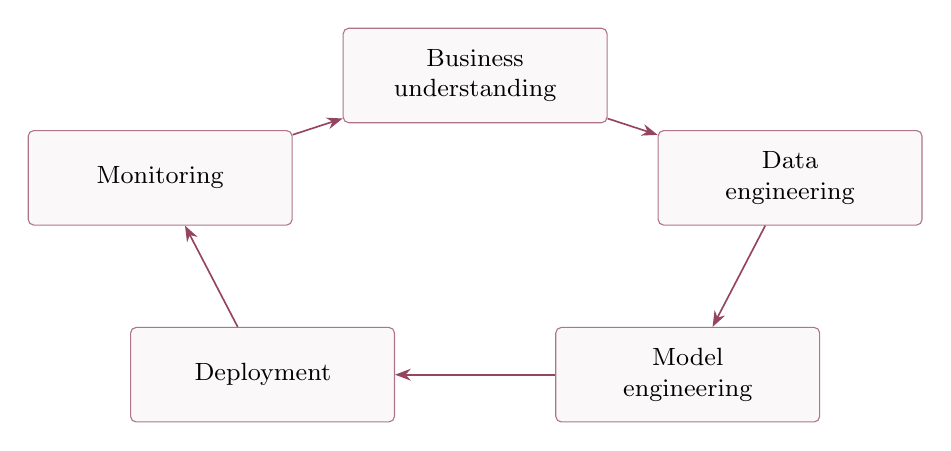
\begin{tikzpicture}
  \node[concept node] (business) at (0,2.1) {Business\\understanding};
  \node[concept node] (data) at (4,0.8) {Data\\engineering};
  \node[concept node] (model) at (2.7,-1.7) {Model\\engineering};
  \node[concept node] (deploy) at (-2.7,-1.7) {Deployment};
  \node[concept node] (monitor) at (-4,0.8) {Monitoring};
  \draw[concept arrow] (business) -- (data);
  \draw[concept arrow] (data) -- (model);
  \draw[concept arrow] (model) -- (deploy);
  \draw[concept arrow] (deploy) -- (monitor);
  \draw[concept arrow] (monitor) -- (business);
\end{tikzpicture}}

\newcommand{\hierarchydiagram}{%
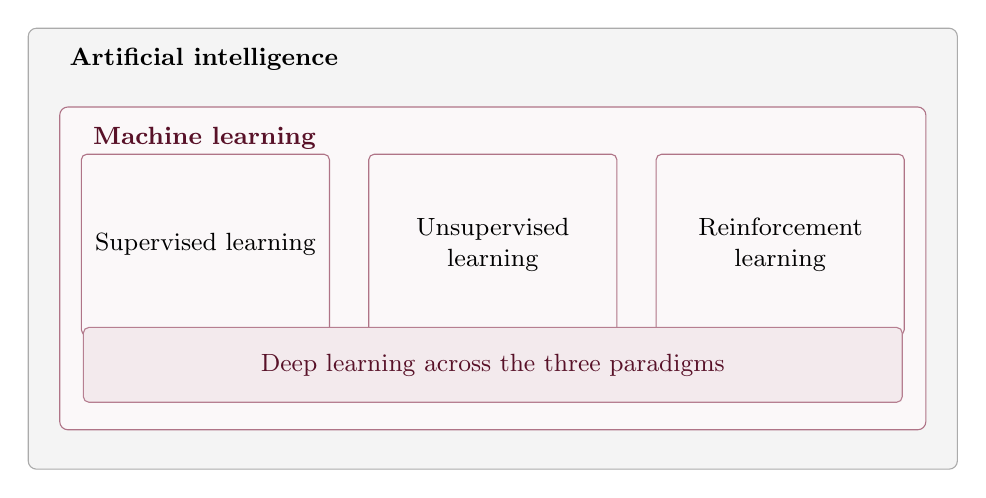
\begin{tikzpicture}[font=\small]
  \draw[draw=MidGray!55,fill=SoftGray,rounded corners=3pt] (-0.4,-0.5) rectangle (11.4,5.1);
  \node[anchor=west,font=\small\bfseries] at (0,4.7) {Artificial intelligence};
  \draw[draw=Sapienza!60,fill=Sapienza!3,rounded corners=3pt] (0,0) rectangle (11,4.1);
  \node[anchor=west,font=\small\bfseries,text=SapienzaDark] at (0.3,3.7) {Machine learning};
  \foreach \x/\name in {1.85/Supervised learning,5.5/Unsupervised learning,9.15/Reinforcement learning}{
    \node[concept node,text width=28mm,minimum height=23mm] at (\x,2.35) {\name};
  }
  \draw[draw=Sapienza!55,fill=Sapienza!9,rounded corners=2pt] (0.3,0.35) rectangle (10.7,1.3);
  \node[text=SapienzaDark] at (5.5,0.82) {Deep learning across the three paradigms};
\end{tikzpicture}}

\newcommand{\programmingdiagram}{%
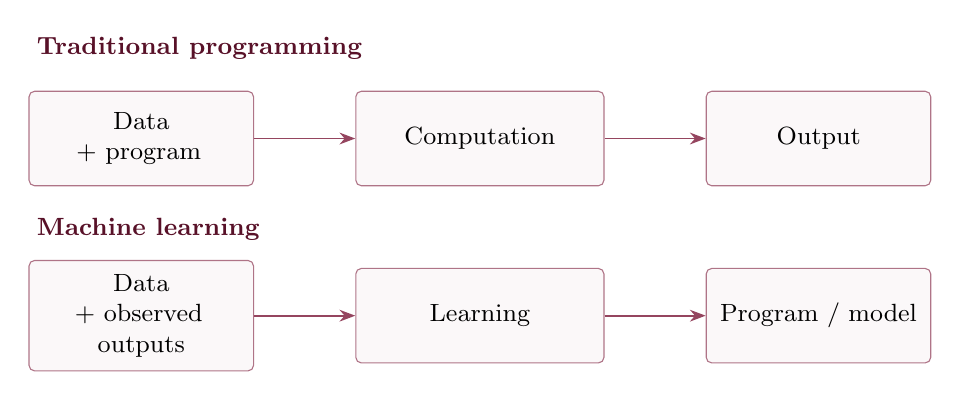
\begin{tikzpicture}[font=\small]
  \node[concept node,text width=25mm] (a) at (0,0) {Data\\+ program};
  \node[concept node,text width=28mm] (b) at (4.3,0) {Computation};
  \node[concept node,text width=25mm] (c) at (8.6,0) {Output};
  \draw[concept arrow] (a) -- (b); \draw[concept arrow] (b) -- (c);
  \node[anchor=west,font=\small\bfseries,text=SapienzaDark] at (-1.45,1.15) {Traditional programming};
  \node[concept node,text width=25mm] (d) at (0,-2.25) {Data\\+ observed outputs};
  \node[concept node,text width=28mm] (e) at (4.3,-2.25) {Learning};
  \node[concept node,text width=25mm] (f) at (8.6,-2.25) {Program / model};
  \draw[concept arrow] (d) -- (e); \draw[concept arrow] (e) -- (f);
  \node[anchor=west,font=\small\bfseries,text=SapienzaDark] at (-1.45,-1.15) {Machine learning};
\end{tikzpicture}}


\begin{document}
\hypersetup{pageanchor=false}

% ============================================================
% TITLE PAGE
% ============================================================
\begin{titlepage}
\thispagestyle{empty}
\centering
\vspace*{1.2cm}

\includegraphics[width=7.2cm]{sapienza-logo.png}\par
\vspace{2.1cm}
{\color{Sapienza}\rule{\textwidth}{0.55pt}\par}
\vspace{1.0cm}
{\fontsize{25}{31}\selectfont\bfseries\color{SapienzaDark}
FOUNDATIONS\par OF DATA SCIENCE\par}
\vspace{0.65cm}
{\large Comprehensive Study Notes\par}
\vspace{1.0cm}
{\color{Sapienza}\rule{\textwidth}{0.55pt}\par}
\vspace{1.9cm}
{\large\instructorname\par}
\vspace{0.35cm}
Department of Computer Science\par
\university\par
\vspace{1.65cm}
{\small\scshape\color{MidGray}Notes prepared by\par}
\vspace{0.25cm}
{\large Matt Clifford Trinidad Ramos\par}
\vfill
{\small\color{MidGray}Calculus and linear algebra\enspace\textperiodcentered\enspace Probability and statistics\par}
\end{titlepage}

\pagenumbering{roman}
\hypersetup{pageanchor=true}
\begingroup
\small
\setlength{\parskip}{0pt}
\tableofcontents
\endgroup
\clearpage
\pagenumbering{arabic}

% ============================================================
% PART I
% ============================================================
\partopening{Data Science and Machine Learning Foundations}

\section{What Is Data Science?}

\begin{definitionbox}
\textbf{Data science} is an interdisciplinary field concerned with extracting actionable insight and knowledge from structured and unstructured data, using methods from statistics, mathematics, computer science, and domain expertise.
\end{definitionbox}

\textbf{Prerequisites.} Calculus and linear algebra (including derivatives and matrix--vector products), and basic probability and statistics (including Gaussian distributions, mean, and standard deviation).

Data science is broader than model fitting. A typical lifecycle starts from the problem that needs to be solved, passes through data and model development, and continues after deployment because models must be monitored and may need retraining.

\begin{figure}[htbp]
\centering\lifecyclediagram
\caption{Data science lifecycle from business understanding through data engineering, model engineering, deployment, and monitoring. Feedback from monitoring initiates a new development cycle.}
\end{figure}

The stages involve the following activities:
\begin{itemize}
  \item \textbf{Business understanding:} define business objectives and translate them into machine-learning objectives.
  \item \textbf{Data engineering:} collect and verify data, clean and visualize it, augment it when appropriate, and standardize it.
  \item \textbf{Model engineering:} select a model, train it, and evaluate it.
  \item \textbf{Deployment:} move the model into production and consider user acceptance and usability.
  \item \textbf{Monitoring:} monitor efficacy, collect new data, and retrain when required.
\end{itemize}

\section{Machine Learning as a Subfield of AI}
Artificial Intelligence (AI) is the field of computer science devoted to creating agents capable of tasks that typically require human intelligence, such as learning, reasoning, and problem solving. Supervised learning, unsupervised learning, and reinforcement learning are major machine-learning paradigms within AI. Deep learning cuts across these paradigms.

\begin{figure}[htbp]
\centering\hierarchydiagram
\caption{Artificial intelligence, machine learning, and the three learning paradigms. Deep learning supplies model families across the paradigms; the diagram is conceptual rather than a strict set-theoretic taxonomy.}
\end{figure}

\subsection{Tom Mitchell's learning-task formulation}
In Tom Mitchell's learning-task formulation, a machine-learning system improves its \textbf{performance} $P$ at a \textbf{task} $T$ through \textbf{experience} $E$. A well-defined learning problem can therefore be summarized by the triple
\[
\langle P,T,E\rangle.
\]

\begin{formulabox}
$T$ denotes the task to be performed; $P$ is the quantitative performance measure; $E$ is the experience or data from which the system learns.
\end{formulabox}

\begin{table}[htbp]
\centering
\caption{Examples of tasks, performance measures, and learning experience.}
\small
\begin{tabularx}{\textwidth}{@{}>{\raggedright\arraybackslash}p{0.24\textwidth}YY@{}}
\toprule
\textbf{Task $T$} & \textbf{Performance $P$} & \textbf{Experience $E$}\\
\midrule
Playing checkers & Percentage of games won against an arbitrary opponent & Practice games played against itself\\
Recognizing handwritten words & Percentage of words correctly classified & Human-labeled images of handwritten words\\
Driving on four-lane highways using vision sensors & Average distance traveled before a human-judged error & Images and steering commands recorded while observing a human driver\\
Classifying email as spam or legitimate & Percentage of messages correctly classified & A database of emails with human-provided labels\\
\bottomrule
\end{tabularx}
\end{table}

\subsection{Why machine learning?}
Many useful tasks are too complex to specify with explicit hand-written rules. Object recognition, speech understanding, and natural-language processing are canonical examples. Instead of manually encoding all rules, machine-learning systems learn useful regularities automatically from data or experience.

\subsection{Machine learning and statistics}
Statistics and machine learning share substantial mathematical and methodological foundations: both fields uncover patterns in data, rely on calculus, probability, and linear algebra, and share many algorithms. Their differences lie mainly in emphasis: statistics traditionally focuses more strongly on inference, conclusions, interpretability, and rigor, whereas machine learning often emphasizes prediction, scalability, and autonomy. These differences in goals and emphasis do not establish a hard boundary between the disciplines.

\section{Learning Paradigms}

\begin{table}[htbp]
\centering
\caption{Input/output view of the three paradigms.}
\begin{tabularx}{\textwidth}{@{}p{0.20\textwidth}YY@{}}
\toprule
\textbf{Paradigm} & \textbf{Input} & \textbf{Output}\\
\midrule
Supervised learning & Examples of inputs paired with desired outputs & A model that predicts an output for a new input\\
Unsupervised learning & Examples of data without target outputs & A representation of structure in the data\\
Reinforcement learning & A sequence of interactions with an environment & A policy that performs a desired task\\
\bottomrule
\end{tabularx}
\end{table}

\section{Supervised Learning}
Supervised learning defines a mapping from input to output and learns this mapping from paired input/output examples. In traditional programming, \emph{data + program} produce the output; in machine learning, \emph{data + observed outputs} are used to learn the program/model.

\begin{figure}[htbp]
\centering\programmingdiagram
\caption{Traditional programming and machine learning: a program computes outputs, whereas learning uses observed inputs and outputs to construct a model.}
\end{figure}

\section{Representative Supervised-Learning Tasks}
A common prediction pipeline encodes raw real-world objects numerically, processes them with a model, and decodes the results into meaningful outputs. The examples differ primarily in the structure and dimensionality of the target.

\subsection{Regression}
Regression predicts real-valued quantities. In the univariate example, real-estate information is encoded as a feature vector and mapped to a single predicted price. In the graph-regression example, a molecular graph is encoded and mapped to more than one continuous target, namely physical properties such as freezing and boiling point.

\academicfigure[0.98\textwidth]{regression.png}{Univariate regression example: a real-world description is encoded numerically and mapped to a single real-valued output.}
\academicfigure[0.98\textwidth]{graph_regression.png}{Graph regression example: a molecular structure is represented numerically and mapped to multiple continuous outputs.}

\subsection{Classification}
Classification predicts discrete classes. A binary text-classification example assigns a sentence to one of two classes (positive/negative) using a Transformer. A music-genre example and an image-classification example illustrate multiclass prediction using, respectively, a recurrent neural network (RNN) and a convolutional network.

\academicfigure[0.98\textwidth]{text_classification.png}{Binary text classification: text $\rightarrow$ numerical representation $\rightarrow$ class scores $\rightarrow$ positive/negative label.}
\academicfigure[0.98\textwidth]{music_classification.png}{Multiclass music-genre classification using a recurrent neural network.}
\academicfigure[0.98\textwidth]{image_classification.png}{Multiclass image classification using a convolutional network.}

\subsection{A supervised model as a family of equations}
A supervised model can predict height from age. Training means searching through a family of candidate equations and selecting one that fits the training observations well. Deep neural networks form extremely flexible families of equations; fitting such networks is an instance of \textbf{deep learning}.

\academicfigure[0.88\textwidth]{supervised_model.png}{Supervised-learning view of model fitting: an input value is mapped to an output through an equation fitted to training data.}

\subsection{Structured and high-dimensional outputs}
Some supervised tasks produce many outputs rather than a single scalar. Examples include:
\begin{itemize}
  \item \textbf{Image segmentation:} many binary/discrete outputs, one per spatial location; the example uses a convolutional encoder--decoder network.
  \item \textbf{Depth estimation:} many continuous outputs forming a dense depth map; using a convolutional encoder--decoder.
  \item \textbf{Pose estimation:} many continuous outputs describing body/keypoint geometry; using a convolutional encoder--decoder.
\end{itemize}

\academicfigure[0.98\textwidth]{image_segmentation.png}{Image segmentation example: an input image is mapped to a dense discrete mask.}
\academicfigure[0.98\textwidth]{depth_estimation.png}{Depth estimation example: an input image is mapped to a dense continuous depth representation.}
\academicfigure[0.98\textwidth]{pose_estimation.png}{Pose estimation example: an input image is mapped to multiple continuous outputs representing pose.}

\subsection{Sequence and cross-modal generation}
The same input--model--output pattern extends to structured sequences and multimodal tasks. Examples include machine translation (text sequence to text sequence), image captioning (image to text sequence), and text-to-image generation (text sequence to image).

\academicfigure[0.98\textwidth]{translation.png}{Machine-translation example: text is tokenized to a numerical representation and decoded into a target-language sequence.}
\academicfigure[0.98\textwidth]{image_captioning.png}{Image-captioning example: an image is encoded numerically and decoded into a textual description.}
\academicfigure[0.98\textwidth]{text_to_image.png}{Text-to-image example: a text prompt is encoded and transformed into an image.}

\FloatBarrier
\begin{keybox}
Across these examples, the relationship between input and output can be highly complex and there may be multiple valid outputs. Nevertheless, outputs---and often inputs---possess structure: language follows grammatical rules and natural images obey strong statistical regularities. This observation motivates learning the ``grammar'' of data from large quantities of unlabeled examples.
\end{keybox}

\section{Unsupervised Learning and Generative Models}
Unsupervised learning studies datasets without target labels. Representative goals include clustering, outlier detection, generation of new examples, and filling in missing data.

A central idea is to exploit the abundance of unlabeled data to learn structure before or alongside a supervised task. An example is \emph{DeepCluster: Deep Clustering for Unsupervised Learning of Visual Features} (Caron et al., 2018), where visual examples are organized into coherent feature clusters without conventional class labels.

\academicfigure[0.88\textwidth]{deepcluster.png}{DeepCluster: visually coherent groups discovered from unlabeled images. The panels illustrate visually coherent groups discovered from unlabeled images.}

\textbf{Generative models} can create new examples. Approaches include generative adversarial networks (GANs), as well as probabilistic generative models such as variational autoencoders (VAEs), normalizing flows, and diffusion models.


\academicfigure[0.78\textwidth]{generative_cats.png}{Examples of synthetic cat images produced by generative models.}

\subsection{Latent variables}
A latent-variable generative model represents high-dimensional observed data through lower-dimensional latent variables. Samples are drawn in the latent space, transformed by the model, and decoded into observations.

\academicfigure[0.83\textwidth]{latent_variables.png}{Latent-variable generation: low-dimensional latent samples are transformed by a deep model into high-dimensional observed data.}

\section{Reinforcement Learning}
Reinforcement learning (RL) involves three basic ingredients: a set of \textbf{states}, a set of \textbf{actions}, and a set of \textbf{rewards}. The agent acts in the environment, changes state, and seeks behavior that produces reward. Unlike ordinary supervised learning, the agent is not given a fixed labeled dataset in advance; it must gather information through interaction.

\subsection{Chess as an example}
In chess, states are valid chess positions and available actions are valid moves. An illustrative reward scheme assigns positive rewards for taking pieces and negative rewards for losing them.

\academicfigure[0.90\textwidth]{rl_chess.png}{Reinforcement-learning pipeline for chess: board state $\rightarrow$ model representation $\rightarrow$ action scores $\rightarrow$ selected move.}

\begin{remarkbox}
Piece-capture rewards illustrate \textbf{reward shaping}: intermediate rewards provide feedback during the state--action--reward interaction loop.
\end{remarkbox}

\subsection{Why reinforcement learning is difficult}
Three central difficulties are:
\begin{itemize}
  \item \textbf{Stochasticity:} the same action need not lead to the same future because other agents or the environment may behave differently.
  \item \textbf{Temporal credit assignment:} a reward observed now may be caused by an earlier sequence of decisions rather than the most recent action alone.
  \item \textbf{Exploration--exploitation trade-off:} an agent must decide whether to reuse a known good strategy or explore alternatives that might be better.
\end{itemize}

\Needspace{30\baselineskip}
\section{Deep-Learning Landmarks}
Yoshua Bengio, Geoffrey Hinton, and Yann LeCun received the 2018 ACM A.M. Turing Award. The following timeline summarizes influential developments in neural networks and deep learning.

\begin{table}[H]
\centering
\caption{Selected milestones in neural networks and deep learning.}
\small
\begin{tabularx}{\textwidth}{@{}C{1.5cm}Y@{}}
\toprule
\textbf{Year} & \textbf{Milestone}\\
\midrule
1958 & Perceptron (simple neural model)\\
1986 & Backpropagation (practical deep neural networks)\\
1989 & Convolutional networks (supervised learning)\\
2012 & AlexNet image classification (supervised learning)\\
2014 & Generative adversarial networks (unsupervised learning)\\
2014 & Deep Q-learning for Atari games (reinforcement learning)\\
2016 & AlphaGo (reinforcement learning)\\
2017 & Machine translation (supervised learning)\\
2019 & Language models (supervised/unsupervised learning)\\
2022 & DALL-E 2, image synthesis from text prompts\\
2022 & ChatGPT\\
2023 & GPT-4 multimodal model\\
2024 & Demis Hassabis and John Jumper: Nobel Prize in Chemistry in connection with AlphaFold-related work; Geoffrey Hinton and John Hopfield: Nobel Prize in Physics\\
2026 & OpenAI announced an AI-generated proof concerning the Navier--Stokes Millennium problem; formal acceptance remains a separate matter.\\
\bottomrule
\end{tabularx}
\end{table}

\noindent{\small\textbf{Historical note (2 October 2026).}
OpenAI announced the proof on 8 September 2026; this announcement does not by itself establish a finalized Millennium Prize determination.
See \href{https://openai.com/index/navier-stokes-solution/}{OpenAI's announcement} and the \href{https://www.claymath.org/millennium/Navier-Stokes-Equation/}{Clay Mathematics Institute's problem page}.}

\begin{keybox}[title=Machine Learning Foundations --- Key Takeaways]
\begin{itemize}
  \item Data science covers the full lifecycle from problem definition and data preparation to deployment and monitoring.
  \item Machine learning replaces explicit hand-coded rules with models learned from data or interaction.
  \item Supervised, unsupervised, and reinforcement learning differ primarily in the information available during learning and the object being learned.
  \item Deep learning supplies highly flexible model families that can be used across several learning paradigms.
  \item Modern tasks often involve structured, high-dimensional inputs and outputs rather than simple scalar prediction.
\end{itemize}
\end{keybox}

% ============================================================
% PART II
% ============================================================
\partopening{Data Representation and Linear Algebra Foundations}

\section{The Iris Dataset and Supervised-Learning Data}
Fisher's Iris dataset provides a compact supervised-learning example. It contains \textbf{150 flowers}: 50 \emph{setosa}, 50 \emph{versicolor}, and 50 \emph{virginica}. Each flower is described by four measurements in centimeters: sepal length, sepal width, petal length, and petal width. The target is the iris species.

\academicfigure[0.63\textwidth]{iris.png}{The three Iris species: versicolor, virginica, and setosa. The classification task predicts the species from sepal and petal measurements.}

\subsection{Features and target}
For $n$ observed objects, the \textbf{features} are properties used to describe each object, while the \textbf{target} is the output variable or prediction goal. Supervised learning assumes that some relationship exists between features and target and attempts to learn a predictive rule from observed examples.

\begin{table}[htbp]
\centering
\caption{Illustrative Iris data: four measurements in centimeters and the species label.}
\begin{tabular}{@{}rrrrl@{}}
\toprule
\textbf{Sepal L.} & \textbf{Sepal W.} & \textbf{Petal L.} & \textbf{Petal W.} & \textbf{Species}\\
\midrule
4.3 & 3.0 & 1.1 & 0.1 & setosa\\
5.0 & 3.3 & 1.4 & 0.2 & setosa\\
7.7 & 3.8 & 6.7 & 2.2 & virginica\\
5.5 & 2.5 & 4.0 & 1.3 & versicolor\\
\bottomrule
\end{tabular}
\end{table}

\subsection{Data types and numerical encoding}
Features and targets can have different types:
\begin{itemize}
  \item numerical variables in $\R$;
  \item integer variables in $\Z$;
  \item categorical variables taking values in a finite set $\{C_1,\ldots,C_g\}$;
  \item binary variables in $\{0,1\}$.
\end{itemize}
For target variables, the distinction between continuous and discrete values leads naturally to regression and classification tasks.

Most learning algorithms expect numerical input. A categorical variable with $k$ mutually exclusive categories can be represented by a one-hot vector
\begin{equation}
\vect e_i=(0,\ldots,0,\underbrace{1}_{i\text{-th position}},0,\ldots,0)^\top,
\qquad i\in\{1,\ldots,k\}.
\label{eq:onehot}
\end{equation}
For categories with a natural order, an encoding should reflect that ordinality, for example through an ordered sequence of integers.

\begin{formulabox}
In \cref{eq:onehot}, $k$ is the number of categories and $\vect e_i$ is the binary indicator for category $i$; exactly one coordinate equals 1.
\end{formulabox}

\subsection{Labels and dataset notation}
Entries in the target column are called \textbf{labels}. Data are \textbf{labeled} when the target is observed and \textbf{unlabeled} when it is unknown.

Let $X$ be the input space and $Y$ the output/target space, with $X\subseteq\R^p$ in the typical vector-valued case. The dataset is written
\begin{equation}
D=\{(\vect x^{(1)},y^{(1)}),\ldots,(\vect x^{(n)},y^{(n)})\}\subset (X\times Y)^n.
\label{eq:dataset}
\end{equation}
Each observation satisfies
\begin{equation}
(\vect x^{(i)},y^{(i)})\in X\times Y,\qquad i=1,\ldots,n,
\end{equation}
and the $j$-th feature column can be represented as
\begin{equation}
\vect x_j=\bigl(x_j^{(1)},\ldots,x_j^{(n)}\bigr)^\top\in\R^n.
\label{eq:feature-column}
\end{equation}

\begin{formulabox}
$n$ is the number of observations; $p$ is the number of input features; $\vect x^{(i)}$ is the feature vector for observation $i$; $y^{(i)}$ is its target; and $\vect x_j$ collects feature $j$ across all $n$ observations.
\end{formulabox}

\section{Data Generation and the i.i.d. Assumption}
The observed dataset $D$ is assumed to arise from an underlying probability distribution $P_{XY}$ defined on $X\times Y$. The true distribution is generally unknown. Supervised machine learning seeks to learn enough of its structure to predict $y$ from $\vect x$.

A standard assumption is that samples are drawn independently and identically distributed (\iid{}) from $P_{XY}$. This contains two assumptions:
\begin{enumerate}
  \item \textbf{Identically distributed:} every sample follows the same underlying distribution.
  \item \textbf{Independent:} the realization of one observation does not depend on the other $n-1$ observations.
\end{enumerate}
This is a strong assumption and may fail in more complex settings such as time series.

\section{Data Points as Vectors}
For vector representations in the input space $X$, assume that the dataset has been \textbf{mean-centered}: the mean along each input dimension is subtracted so that the data cloud is centered around the origin. This operation is reversible as long as the feature means are retained.

Each observation can then be viewed as a point---equivalently, a vector---in a multidimensional vector space. A vector space is a collection of vectors closed under vector addition and scalar multiplication.

\academicfigure[0.72\textwidth]{vectors_visual.png}{Two equivalent visualizations of the same 2-D data: points (left) and arrows from the origin (right).}

\section{Spanning Sets and Bases}
\subsection{Spanning sets}
\begin{definitionbox}
A \textbf{spanning set} is a collection of vectors whose linear combinations can produce every vector in the space being spanned.
\end{definitionbox}

In two dimensions, the standard vectors
\[
\vect e_1=\begin{bmatrix}1\\0\end{bmatrix},\qquad
\vect e_2=\begin{bmatrix}0\\1\end{bmatrix}
\]
span the plane because any point $\begin{bmatrix}x&y\end{bmatrix}^\top$ can be written as
\begin{equation}
\begin{bmatrix}x\\y\end{bmatrix}=x\vect e_1+y\vect e_2.
\end{equation}

\subsection{Basis}
\begin{definitionbox}
A \textbf{basis} is a linearly independent spanning set. In an $N$-dimensional vector space, a basis therefore contains exactly $N$ vectors. A more general spanning set may contain more than $N$ vectors, but then it is not a basis in the minimal sense.
\end{definitionbox}

For a candidate basis $\vect c_1,\ldots,\vect c_N$ and each data point $\vect x_p$, perfect representation means that there are weights $w_{1,p},\ldots,w_{N,p}$ such that
\begin{equation}
\sum_{n=1}^{N}\vect c_n w_{n,p}=\vect x_p,
\qquad p=1,\ldots,P.
\label{eq:basis-representation}
\end{equation}

\begin{formulabox}
$N$ is the ambient dimension; $P$ is the number of data points; $\vect c_n$ is basis vector $n$; $w_{n,p}$ is the coordinate/weight of data point $p$ along $\vect c_n$; $\vect x_p$ is the original point.
\end{formulabox}

\academicfigure[0.78\textwidth]{basis_visual.png}{Points, vectors from the origin, and a basis representation in two dimensions.}

\section{Standard and Orthonormal Bases}

\subsection{The standard basis}
The $k$-th standard basis vector has zeros everywhere except for a 1 in position $k$:
\[
\vect c_k=(0,\ldots,0,1,0,\ldots,0)^\top.
\]
For distinct basis vectors, the inner product is zero, while each vector has unit Euclidean norm:
\begin{align}
\vect c_n^\top \vect c_m &=0, && n\neq m,\\
\|\vect c_n\|_2^2&=1, && n=1,\ldots,N.
\end{align}
Thus the standard basis is orthonormal. If
\[
C=[\vect c_1\;\vect c_2\;\cdots\;\vect c_N],
\]
then
\begin{equation}
C^\top C=I_{N\times N}.
\label{eq:orthonormal}
\end{equation}
In the standard basis, the coordinate vector of a point is simply the point itself: $\vect w_p=\vect x_p$.

\academicfigure[0.48\textwidth]{standard_basis_example.png}{Reconstruction in the two-dimensional standard basis: a point $(5,5)$ is reconstructed from weights $w_1=5$ and $w_2=5$.}

\subsection{Encoding with an orthonormal basis}
For an orthonormal basis, the encoding of $\vect x_p$ is obtained directly by inner products:
\begin{equation}
\vect w_p=C^\top \vect x_p,
\qquad p=1,\ldots,P.
\label{eq:orthonormal-encoding}
\end{equation}
Reconstruction is exact when $C$ is a complete $N\times N$ orthonormal basis:
\begin{equation}
CC^\top\vect x_p=\vect x_p,
\qquad p=1,\ldots,P.
\label{eq:orthonormal-reconstruction}
\end{equation}

\begin{formulabox}
$C$ contains the orthonormal basis vectors as columns; $C^\top\vect x_p$ produces the coordinate vector $\vect w_p$; multiplying by $C$ decodes the coordinates back into the original data space.
\end{formulabox}

\section{Non-Standard Bases and Coordinate Transformations}
For a non-standard basis, the coordinate vector generally differs numerically from the original data point. The encoding is
\begin{equation}
\vect w_p=
\begin{bmatrix}
w_{1,p}\\w_{2,p}\\\vdots\\w_{N,p}
\end{bmatrix},
\end{equation}
which represents $\vect x_p$ in a transformed feature space whose coordinate axes are defined by the spanning vectors.

Consider the basis vectors
\begin{equation}
\vect c_1=\begin{bmatrix}2\\1\end{bmatrix},
\qquad
\vect c_2=\begin{bmatrix}1\\2\end{bmatrix}.
\label{eq:nonstandard-vectors}
\end{equation}
Because these vectors are linearly independent, any point in $\R^2$ can be expressed uniquely as
\begin{equation}
w_{1,p}\vect c_1+w_{2,p}\vect c_2=\vect x_p.
\label{eq:nonstandard-representation}
\end{equation}

\academicfigure[0.75\textwidth]{nonstandard_basis_example.png}{A point $\vect x_1$ in the original coordinates (left) and its encoding $\vect w_1$ in coordinates defined by the non-standard basis (right).}
\academicfigure[0.78\textwidth]{nonstandard_weights.png}{Geometric decomposition in a non-standard basis: the red vector is reconstructed from scaled basis vectors, while the coordinate vector records the required weights.}

\section{Finding the Encoding Weights}
Let the basis/spanning vectors be stacked column-wise into
\begin{equation}
C=[\vect c_1\;\vect c_2\;\cdots\;\vect c_N],
\end{equation}
and let $\vect w_p$ contain the weights for point $\vect x_p$. The squared reconstruction cost is
\begin{equation}
h(\vect w_p)=\|C\vect w_p-\vect x_p\|_2^2.
\label{eq:reconstruction-cost}
\end{equation}
Setting the gradient to zero yields the symmetric first-order system
\begin{equation}
C^\top C\vect w_p=C^\top\vect x_p,
\qquad p=1,\ldots,P.
\label{eq:normal-equations}
\end{equation}
For all $P$ points together, the optimization problem is
\begin{equation}
\underset{\vect w_1,\vect w_2,\ldots,\vect w_P}{\operatorname{minimize}}
\;\frac{1}{P}\sum_{p=1}^{P}\|C\vect w_p-\vect x_p\|_2^2.
\label{eq:average-reconstruction}
\end{equation}

\begin{formulabox}
$C$ is the matrix of spanning vectors; $\vect w_p$ is the coordinate/encoding vector; $\vect x_p$ is the original point; $h(\vect w_p)$ is squared reconstruction error. Equation~\eqref{eq:normal-equations} is the normal-equation form obtained from the first-order optimality condition.
\end{formulabox}

\academicfigure[0.75\textwidth]{encoded_data.png}{Original data versus the same observations represented in the coordinate system defined by a non-standard spanning set.}

\section{Subspaces and Projection}
Up to this point, perfect representation in a generic $N$-dimensional space requires enough independent spanning directions. If only $K<N$ independent vectors are used, they can span at most a $K$-dimensional subspace of the full $N$-dimensional space. For example, in three dimensions, $K=2$ independent vectors span a plane, while $K=1$ spans a line.

\academicfigure[0.75\textwidth]{subspace_3d.png}{Lower-dimensional subspaces: a line or plane cannot represent every point in the ambient space exactly.}

For $K$ spanning vectors, the matrix now has shape
\[
C=[\vect c_1\;\cdots\;\vect c_K]\in\R^{N\times K},
\]
but the first-order system keeps the same form:
\begin{equation}
C^\top C\vect w_p=C^\top\vect x_p,
\qquad p=1,\ldots,P.
\label{eq:subspace-normal}
\end{equation}

\subsection{Encoding, decoding, and projection}
When $K<N$, the point cannot in general be reconstructed exactly. Instead, encoding maps the point to $K$ coordinates, and decoding combines those coordinates with the $K$ basis vectors to obtain the closest representable point in the subspace. Geometrically, this is an orthogonal \textbf{projection}: dropping the point perpendicularly onto the subspace.

\academicfigure[0.90\textwidth]{encoding_decoding.png}{Encoding and decoding in a lower-dimensional subspace. The decoded point lies in the chosen lower-dimensional subspace and approximates the original point.}

If the $K$ subspace basis vectors are orthonormal, the encoding again simplifies to
\begin{equation}
\vect w_p=C^\top\vect x_p,
\qquad p=1,\ldots,P,
\label{eq:subspace-orth-encoding}
\end{equation}
and decoding gives the orthogonal projection
\begin{equation}
CC^\top\vect x_p\approx \vect x_p,
\qquad p=1,\ldots,P.
\label{eq:projection}
\end{equation}
The approximation becomes equality only when the original point already lies in the spanned subspace (or when the orthonormal set is a complete basis of the whole space).

\begin{formulabox}
For an orthonormal $N\times K$ matrix $C$, $C^\top\vect x_p$ is the $K$-dimensional encoding and $CC^\top\vect x_p$ is the decoded projection in the original $N$-dimensional space. The residual $\|CC^\top\vect x_p-\vect x_p\|_2$ measures the projection/reconstruction error between the original point and its projection.
\end{formulabox}

\academicfigure[0.92\textwidth]{orthonormal_projection.png}{Geometric interpretation of orthonormal projection for one and two basis directions. The residual is perpendicular to the spanned subspace.}

\begin{keybox}[title=Vector Spaces and Projections --- Key Takeaways]
\begin{itemize}
  \item A supervised dataset pairs feature vectors with targets; categorical features often require numerical encoding.
  \item Samples are modeled as independent, identically distributed draws from an unknown joint distribution $P_{XY}$.
  \item A spanning set generates a space through linear combinations; a basis is a minimal linearly independent spanning set.
  \item Orthonormal bases make encoding especially simple: coordinates are inner products, $\vect w=C^\top\vect x$.
  \item A non-standard basis changes coordinates but can still represent the same point exactly when it spans the entire space.
  \item With only $K<N$ directions, decoding produces a projection onto a lower-dimensional subspace rather than an exact reconstruction in general.
\end{itemize}
\end{keybox}

\Needspace{23\baselineskip}
\section{Quick Review and Terminology}
\begin{table}[H]
\centering
\caption{Core concepts in machine learning, data representation, and linear algebra.}
\small
\begin{tabularx}{\textwidth}{@{}p{0.24\textwidth}Y@{}}
\toprule
\textbf{Term} & \textbf{Meaning}\\
\midrule
Feature & Input property describing an observation\\
Target / label & Output variable to be predicted; a label is an observed target entry\\
One-hot encoding & $k$-dimensional binary representation with exactly one active coordinate\\
i.i.d. & Independent and identically distributed sampling assumption\\
Spanning set & Vectors whose linear combinations generate a space/subspace\\
Basis & Linearly independent spanning set; minimal representation of a vector space\\
Orthonormal basis & Basis vectors are mutually orthogonal and have unit norm\\
Encoding & Coordinate vector $\vect w$ representing a point relative to chosen spanning vectors\\
Decoding & Reconstruction $C\vect w$ in the original data space\\
Projection & Closest representable point in a lower-dimensional subspace, illustrated by $CC^\top\vect x$ for an orthonormal subspace basis\\
Supervised learning & Learning a mapping from labeled input/output examples\\
Unsupervised learning & Learning structure from data without target labels\\
Reinforcement learning & Learning a policy through state/action/reward interaction\\
\bottomrule
\end{tabularx}
\end{table}


\section*{References}
\phantomsection
\addcontentsline{toc}{section}{References}
\markboth{References}{}
\begin{enumerate}[label={[\arabic*]},itemsep=0.45em]
  \item Deisenroth, Faisal, and Ong. \emph{Mathematics for Machine Learning}.
  \item Simon Prince. \emph{Understanding Deep Learning}.
  \item Watt, Borhani, and Katsaggelos. \emph{Machine Learning Refined}, Chapter 8.
  \item Caron et al. (2018). \emph{DeepCluster: Deep Clustering for Unsupervised Learning of Visual Features}.
  \item 3Blue1Brown. \emph{Essence of Linear Algebra}, video series.
\end{enumerate}
\end{document}
